\section*{Задание}
{
\verbatimFont
Листинг по XAML.
\small
\begin{verbatim}

<Window x:Class="pugin_calc.MainWindow"
        xmlns="http://schemas.microsoft.com/winfx/2006/xaml/presentation"
        xmlns:x="http://schemas.microsoft.com/winfx/2006/xaml"
        xmlns:d="http://schemas.microsoft.com/expression/blend/2008"
        xmlns:mc="http://schemas.openxmlformats.org/markup-compatibility/2006"
        xmlns:local="clr-namespace:pugin_calc"
        mc:Ignorable="d"
        Title="CALC" Height="339.243" Width="517.828">
    <Grid>
        <Grid.ColumnDefinitions>
            <ColumnDefinition Width="136*"/>
            <ColumnDefinition Width="3*"/>
            <ColumnDefinition Width="22*"/>
            <ColumnDefinition Width="94*"/>
        </Grid.ColumnDefinitions>
        <Button Content="X^2" HorizontalAlignment="Left" Margin="27,126,0,0"
 VerticalAlignment="Top" Width="75" Background="White" BorderBrush="Black"
 FontFamily="Open Sans" FontSize="16" Height="50" Click="Button_Click_18"/>
        <Button Content="1" HorizontalAlignment="Left" Margin="103,126,0,0"
 VerticalAlignment="Top" Width="75" Background="White" BorderBrush="Black"
 FontFamily="Open Sans" FontSize="11" Height="50" Click="Button_Click_6"/>
        <Button Content="Button" HorizontalAlignment="Left"
 Margin="179,177,0,0" VerticalAlignment="Top" Width="75" Background="White"
 BorderBrush="Black" FontFamily="Open Sans" FontSize="11" Height="50"/>
        <Button Content="2" HorizontalAlignment="Left" Margin="179,126,0,0"

 VerticalAlignment="Top" Width="75" Background="White" BorderBrush="Black"
 FontFamily="Open Sans" FontSize="11" Height="50" Click="Button_Click_7"/>
        <Button Content="Button" HorizontalAlignment="Left"

 Margin="27,177,0,0" VerticalAlignment="Top" Width="75" Background="White"
 BorderBrush="Black" FontFamily="Open Sans" FontSize="11" Height="50"/>
        <Button Content="Button" HorizontalAlignment="Left"
 Margin="103,177,0,0" VerticalAlignment="Top" Width="75" Background="White"
 BorderBrush="Black" FontFamily="Open Sans" FontSize="11" Height="50"/>

        <Button Content="3" HorizontalAlignment="Left" Margin="255,126,0,0"
 VerticalAlignment="Top" Width="74" Background="White" BorderBrush="Black"
 FontFamily="Open Sans" FontSize="11" Height="50" Grid.ColumnSpan="4"

 Click="Button_Click_8"/>
        <Button Content="корень" HorizontalAlignment="Left"
 Margin="13,126,0,0" VerticalAlignment="Top" Width="75"
 Background="White" BorderBrush="Black" FontFamily="Open Sans" FontSize="11"
 Height="50" Grid.Column="3" Click="Button_Click_19"/>
        <Button Content="=" HorizontalAlignment="Left" Margin="89,126,0,0"
 VerticalAlignment="Top" Width="75" BorderBrush="Black" FontFamily="Open
 Sans" FontSize="36" Height="101" Foreground="Black" Background="White"
 Grid.Column="3" Click="Button_Click_1"/>
        <Button Content="Button" HorizontalAlignment="Left"
 Margin="255,177,0,0" VerticalAlignment="Top" Width="74"
 Background="White" BorderBrush="Black" FontFamily="Open Sans" FontSize="11"
 Height="50" Grid.ColumnSpan="4"/>
        <Button Content="Button" HorizontalAlignment="Left"
 Margin="13,177,0,0" VerticalAlignment="Top" Width="75"
 Background="White" BorderBrush="Black" FontFamily="Open Sans" FontSize="11"
 Height="50" Grid.Column="3"/>
        <Button Content="C"  HorizontalAlignment="Left" Margin="28,75,0,0"
 VerticalAlignment="Top" Width="150" BorderBrush="Black" FontFamily="Open
 Sans" FontSize="20" Height="50" Background="White" Click="Button_Click_17"/>
        <Button Content="+" HorizontalAlignment="Left" Margin="179,75,0,0"
 VerticalAlignment="Top" Width="75" Background="White" BorderBrush="Black"
 FontFamily="Open Sans" FontSize="20" Height="50" Click="Button_Click_2"/>
        <Button Content="-" HorizontalAlignment="Left" Margin="255,75,0,0"
 VerticalAlignment="Top" Width="74" Background="White"
 BorderBrush="Black" FontFamily="Open Sans" FontSize="20" Height="50"
 Grid.ColumnSpan="4" Click="Button_Click_3"/>
        <Button Content="*" HorizontalAlignment="Left" Margin="13,75,0,0"
 VerticalAlignment="Top" Width="75" Background="White" BorderBrush="Black"
 FontFamily="Open Sans" FontSize="20" Height="50" Grid.Column="3"
 Click="Button_Click_4"/>
        <Button Content="/" HorizontalAlignment="Left" Margin="89,75,0,0"
 VerticalAlignment="Top" Width="75" Background="White" BorderBrush="Black"
 FontFamily="Open Sans" FontSize="20" Height="50" Grid.Column="3"
 Click="Button_Click_5"/>
        <TextBox Name="FieldCalc"  HorizontalAlignment="Left" Height="38"
 Margin="27,19,0,0" TextWrapping="Wrap" VerticalAlignment="Top" Width="460"
 FontFamily="Open Sans" FontSize="16" Padding="5" Grid.ColumnSpan="4"
 IsEnabled="False" Background="White" Foreground="Black"

 SelectionBrush="Black"/>
        <Button Content="5" HorizontalAlignment="Left" Margin="179,177,0,0"
 VerticalAlignment="Top" Width="75" Background="White" BorderBrush="Black"
 FontFamily="Open Sans" FontSize="11" Height="50" Click="Button_Click_10"/>
        <Button Content="." HorizontalAlignment="Left" Margin="27,177,0,0"
 VerticalAlignment="Top" Width="75" Background="White" BorderBrush="Black"
 FontFamily="Open Sans" FontSize="11" Height="50" Click="Button_Click_16"/>
        <Button Content="4" HorizontalAlignment="Left" Margin="103,177,0,0"
 VerticalAlignment="Top" Width="75" Background="White" BorderBrush="Black"
 FontFamily="Open Sans" FontSize="11" Height="50" Click="Button_Click_9"/>
        <Button Content="6" HorizontalAlignment="Left" Margin="255,177,0,0"
 VerticalAlignment="Top" Width="74" Background="White" BorderBrush="Black"
 FontFamily="Open Sans" FontSize="11" Height="50" Grid.ColumnSpan="4"
 Click="Button_Click_11"/>
        <Button Content="X^3" HorizontalAlignment="Left" Margin="13,177,0,0"
 VerticalAlignment="Top" Width="75" Background="White" BorderBrush="Black"
 FontFamily="Open Sans" FontSize="16" Height="50" Grid.Column="3"
 Click="Button_Click_20"/>
        <Button Content="8" HorizontalAlignment="Left" Margin="179,228,0,0"
 VerticalAlignment="Top" Width="75" Background="White" BorderBrush="Black"
 FontFamily="Open Sans" FontSize="11" Height="50" Click="Button_Click_13"/>
        <Button Content="0" HorizontalAlignment="Left" Margin="27,228,0,0"
 VerticalAlignment="Top" Width="75" Background="White" BorderBrush="Black"
 FontFamily="Open Sans" FontSize="11" Height="50" Click="Button_Click_15"/>
        <Button Content="7" HorizontalAlignment="Left" Margin="103,228,0,0"
 VerticalAlignment="Top" Width="75" Background="White" BorderBrush="Black"
 FontFamily="Open Sans" FontSize="11" Height="50" Click="Button_Click_12"/>
        <Button Content="9" HorizontalAlignment="Left" Margin="255,228,0,0"
 VerticalAlignment="Top" Width="75" Background="White" BorderBrush="Black"
 FontFamily="Open Sans" FontSize="11" Height="50" Grid.ColumnSpan="4"
 Click="Button_Click_14"/>
        <Button Content="EXIT" HorizontalAlignment="Left"
 Margin="14,228,0,0" VerticalAlignment="Top" Width="151" BorderBrush="Black"
 FontFamily="Open Sans" FontSize="11" Height="50" Foreground="Black"
 Click="Button_Click" Background="White" Grid.Column="3"/>

    </Grid>
</Window>


\end{verbatim}
Листинг по C\# коду
\begin{verbatim}


namespace pugin_calc
{
    /// <summary>
    /// Логика взаимодействия для MainWindow.xaml
    /// </summary>
    public partial class MainWindow : Window
    {
        public MainWindow()
        {
            InitializeComponent();
        }
        public string VariableA = "";
        public string VariableB = "";
        public bool flag = false;//replace variable with value textbox
 (отвечает за смену переменных значений поля)
        public int sign = 0;//number operate(под каждым номером своя операция)
        public bool signPress = false;// answer for press one button + - *
 \(убураем возможность повторного нажатия клавиши)
        public bool point = false;//избавляемся от повтороного нажатия кнопки
        bool press = false;//нужно чтобы проверить что перед нажатием на
 знаки (.) или +-*\ было что то внесено в textbox

        private void Button_Click(object sender, RoutedEventArgs e)
        {
            Close();
        }

        private void Button_Click_1(object sender, RoutedEventArgs e)
        {
            press = true;
            if (sign != 0)//(проверяем выбрана  ли операция над числами)
            {
                press = false;

                double var_a = Convert.ToDouble(VariableA);
                double var_b = Convert.ToDouble(VariableB);

                double c;
                switch (sign)
                {

                    case 1:
                        c = var_a + var_b;
                        FieldCalc.Text = Convert.ToString(c);
                        break;
                    case 2:
                        c = var_a - var_b;
                        FieldCalc.Text = Convert.ToString(c);
                        break;
                    case 3:
                        c = var_a * var_b;
                        FieldCalc.Text = Convert.ToString(c);
                        break;
                    case 4:
                        c = var_a / var_b;
                        FieldCalc.Text = Convert.ToString(c);
                        break;
                    default:
                        c = 0;
                        FieldCalc.Text = Convert.ToString(c);
                        break;
                }

                flag = false;
                signPress = false;
                sign = 0;
                VariableA = c.ToString();
                VariableB = "";
                c = 0;
            }

        }

        private void Button_Click_2(object sender, RoutedEventArgs e)
        {    //addition
            press = false;//елси клавиша нажата то нельзя ничего
 записать не внеся данные 



            if (signPress == false)//если операция ещё не выбрана
            {
                flag = true;// другое значение записываем в другую переменную
                sign = 1;//записываем номер операции
                FieldCalc.Text += " + ";
                signPress = true;//коворим что операция уже выбрана
                point = false;
            }
        }

        private void Button_Click_3(object sender, RoutedEventArgs e)
        {

            press = false;
            //substraction
            if (signPress == false)
            {
                flag = true;
                sign = 2;
                FieldCalc.Text += " - ";
                signPress = true;
                point = false;
            }
        }

        private void Button_Click_4(object sender, RoutedEventArgs e)
        {

            press = false;
            //multiplication
            if (signPress == false)
            {
                flag = true;
                sign = 3;
                FieldCalc.Text += " * ";
                signPress = true;
                point = false;
            }
        }

        private void Button_Click_5(object sender, RoutedEventArgs e)
        {

            press = false;
            //division
            if (signPress == false)
            {
                flag = true;
                sign = 4;
                FieldCalc.Text += " / ";
                signPress = true;
                point = false;
            }
        }

        private void Button_Click_6(object sender, RoutedEventArgs e)
        {
            press = true;
            // press 1
            if (flag == false)
            {
                VariableA += "1";
            }
            else
                VariableB += "1";

            FieldCalc.Text += 1;
        }

        private void Button_Click_7(object sender, RoutedEventArgs e)
        {
            press = true;
            // press 2
            if (flag == false)
            {
                VariableA += "2";
            }
            else
                VariableB += "2";
            FieldCalc.Text += 2;
        }

        private void Button_Click_8(object sender, RoutedEventArgs e)
        {
            press = true;
            // press 3
            if (flag == false)
            {
                VariableA += "3";
            }
            else
                VariableB += "3";
            FieldCalc.Text += 3;
        }

        private void Button_Click_9(object sender, RoutedEventArgs e)
        {
            press = true;
            // press 4
            if (flag == false)
            {
                VariableA += "4";
            }
            else
                VariableB += "4";
            FieldCalc.Text += 4;
        }

        private void Button_Click_10(object sender, RoutedEventArgs e)
        {
            press = true;
            // press 5
            if (flag == false)
            {
                VariableA += "5";
            }
            else
                VariableB += "5";
            FieldCalc.Text += 5;
        }

        private void Button_Click_11(object sender, RoutedEventArgs e)
        {
            press = true;
            // press 6
            if (flag == false)
            {
                VariableA += "6";
            }
            else
                VariableB += "6";
            FieldCalc.Text += 6;
        }

        private void Button_Click_12(object sender, RoutedEventArgs e)
        {
            press = true;
            // press 7
            if (flag == false)
            {
                VariableA += "7";
            }
            else
                VariableB += "7";
            FieldCalc.Text += 7;
        }

        private void Button_Click_13(object sender, RoutedEventArgs e)
        {
            press = true;
            // press 8
            if (flag == false)
            {
                VariableA += "8";
            }
            else
                VariableB += "8";
            FieldCalc.Text += 8;
        }

        private void Button_Click_14(object sender, RoutedEventArgs e)
        {
            press = true;
            // press 9
            if (flag == false)
            {
                VariableA += "9";
            }
            else
                VariableB += "9";
            FieldCalc.Text += 9;
        }

        private void Button_Click_15(object sender, RoutedEventArgs e)
        {
            press = true;
            // press 0
            if (flag == false)
            {
                VariableA += "0";
            }
            else
                VariableB += "0";
            FieldCalc.Text += 0;
        }
        private void Button_Click_16(object sender, RoutedEventArgs e)
        {
            // press
            if (press == true)
            {
                if (point == false)//избавляемся от повтороного нажатия кнопки
                {
                    if (flag == false)
                    {
                        VariableA += ",";
                        // point = true;
                    }
                    point = true;
                    FieldCalc.Text += ".";
                }
            }
        }
        private void Button_Click_17(object sender, RoutedEventArgs e)
        {
            //сброс
            press = false;

            flag = false;
            signPress = false;
            sign = 0;
            VariableA = "";
            VariableB = "";
            point = false;
            FieldCalc.Text = "";
        }
        private void Button_Click_18(object sender, RoutedEventArgs e)
        {
            double a = Convert.ToDouble(VariableA);
            a *= a;
            FieldCalc.Text = Convert.ToString(a);
            VariableA = a.ToString();
        }
        private void Button_Click_19(object sender, RoutedEventArgs e)
        {
            double a = Convert.ToDouble(VariableA);

            FieldCalc.Text = Convert.ToString(Math.Sqrt(a));
            VariableA = a.ToString();}
        private void Button_Click_20(object sender, RoutedEventArgs e)
        {
            double a = Convert.ToDouble(VariableA);
            a = a * (a * a);
            FieldCalc.Text = Convert.ToString(a);
            VariableA = a.ToString();}
        private void delet_chart(object sender, RoutedEventArgs e)
        {
            if (signPress == false)//если операция ещё не выбрана
            {
                string[] a = VariableA.Split();
                for (int i = 0; i <= a.Length - 1; i++)
                {
                }
            }
            else
            {
            }}}}

\end{verbatim}



\begin{figure}[h]
\centering
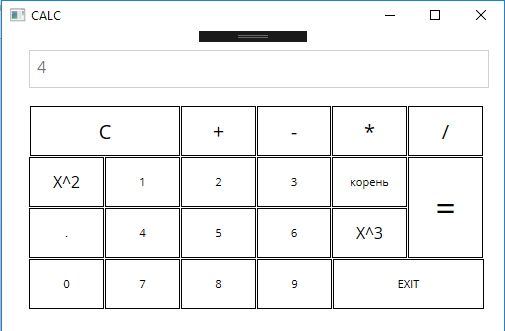
\includegraphics[scale=1]{file1}
\caption{вводим данные}
\label{fig:file1}
\end{figure}

\begin{figure}[h]
\centering
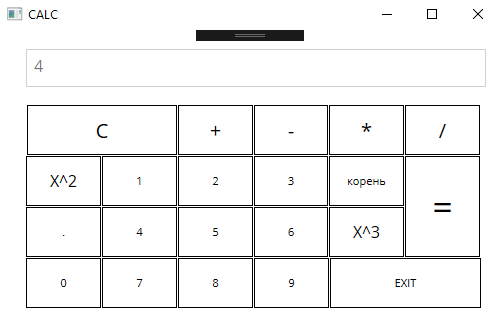
\includegraphics[scale=1]{file2}
\caption{Получаем ответ}
\label{fig:file2}
\end{figure}

